\documentclass{amsart}[12pt]
\usepackage{amsmath, amsfonts, tikz, natbib, array}
\usetikzlibrary{patterns}
\oddsidemargin=0in \evensidemargin=0in
\textwidth=6.6in \textheight=8.7in

\title{Map projections between spherical and Euclidean triangles}
\author{B R S Recht}
\date{April 2020}

\begin{document}
\maketitle
\tableofcontents

\section{Introduction}
A small but persistent trend in creating world maps has been to map onto a
polyhedron, and then unfold the polyhedron into a flat polyhedral net. An
example is Buckminster Fuller's (second) Dymaxion map, based on an
icosahedron.\cite{gray94} Snyder also presented equal-area maps on the
tetrahedron, octahedron, and icosahedron.\cite{snyder92} The inverse mapping of
each map projection can be used to inscribe a regular grid on a sphere, termed
a geodesic grid (after Fuller's geodesic domes) or discrete global
grid.\cite{williamson}\cite{sahr98}. In Buckminster Fuller's construction of
geodesic domes, a method analogus to Fuller's map projection, but not the same,
appears.\cite{kenner}

Discussion of these maps often neglects the projection used to project onto the
polyhedron. In the literature, there are four such map projections
(or families thereof):
\begin{itemize}
\item Gnomonic - Known in antiquity, this map projection preserves geodesics:
  great circle arcs on the sphere are mapped to lines on the plane.
\item Conformal - These map projections preserve the shape of features.
\item Snyder Equal-Area - These map projections preserve the relative area of
  features.\cite{snyder92}
\item Fuller - The map projections derived by Buckminster Fuller
  for his Dymaxion maps.\cite{gray94}\cite{gray95}\cite{crider08}
\end{itemize}
These will be discussed in more detail later on. There are also map projections
in the literature for particular polygons, e.g. the faces of a particular
regular polyhedron, as in Lee's conformal tetrahedral map.\cite{lee} In general
the published projections all fall into one of the categories above.

This paper is limited to triangular faces: projections to quadrilateral faces
or faces with more sides are uncommon, and often involve dividing the face into
triangles. (An interesting exception is the projection in \cite{crider09}, a
quadrilateral projection similar to Fuller's.) Most published projections only
treat regular triangles, although some can be reasonably extended to irregular
triangles. In this text, map projections between spherical and Euclidean
triangles will be discussed. Some of these are existing map projections, or
extensions of those, while some are new compromise map projections. Some
projections where only the forward or inverse transformation is known in close-
form are included. An attempt is made to generalize projections to irregular
triangles and to be able to project a portion of the exterior of the triangle
as well.

\begin{table}
\begin{tabular}[]{p{3.5cm}|p{1.4cm}p{1.4cm}p{1cm}p{7cm}}
  Name & Forward & Inverse & Cite & Notes \\
  Gnomonic & & & \cite{snyder87} & Preserves geodesics  \\
  Conformal & Eq. \ref{eq:conformal} & Eq. \ref{eq:conformal} & \cite{nehari57}\cite{nehari65}& Slow\\
  Snyder Equal-area & & & \cite{snyder92} & New generalization given here\\
  Symmetrized Snyder & & & New & \\
  Areal & & & New &\\
  Fuller & & & \cite{gray94}\cite{gray95} &\\
  Linear Combination & & N/A & New & Parametrized family\\
  Reverse Fuller & N/A & & \cite{kenner} &\\
  Naive Slerp & N/A & Eq. \ref{eq:nst}  & New & Parametrized family\\
\end{tabular}
\caption{Map projections in this text.}
\label{fig:projs}
\end{table}

\section{Preliminaries}
Let $(u,v)$ be a vector in $\mathbb R^2$, and $\zeta = u + i v$ be the
corresponding complex number in $\mathbb C$ or the Riemann sphere $\mathbb C
\cup \{\infty\}$. Which notation is used will depend on the mapping:
conformal maps are best expressed in terms of complex variables.

\subsection{Spherical geometry with 3-vectors}
Some of the map projections to be discussed are better expressed
in terms of a vector rather than latitude and longitude. This text will only
cover pertinent details: a fuller description can be found in e.g. \cite{strang80}.

Let $\phi \in [-\frac{\pi}{2}, \frac{\pi}{2}]$ be latitude, and
$\lambda \in (-\pi, \pi]$ be longitude. Let $\mathbf v = (x, y, z)$ be a vector
in $\mathbb R^3$ and $\mathbf{\hat{v}} = (x, y, z)$ be a unit vector on the
sphere $S^2$ such that $\| \mathbf{\hat{v}} \| = \sqrt{x^2 + y^2 +z^2} = 1$.
To convert from latitude and longitude to a unit vector:
\begin{equation}
  \mathbf{\hat{v}} = \left(\sin (\phi), \sin (\lambda) \cos (\phi),
  -\cos (\lambda) \cos (\phi) \right)
\end{equation}
To convert from the unit vector $\mathbf{\hat{v}}$ to latitude and longitude:
\begin{equation}\begin{split}
  \phi &= \arcsin (x) = \arctan (x, \sqrt{y^2 + z^2}) \\
  \lambda &= \arctan (y, -z)
\end{split}\end{equation}

Often in this text we'll normalize a vector to make it a unit vector.
For brevity,
we'll notate this pre-normalized vector as $\mathbf{\widetilde{v}}$, such that
\begin{equation}
  \mathbf{\hat{v}} = \frac{\mathbf{\widetilde{v}}}{\|\mathbf{\widetilde{v}}\|}
\end{equation}

\subsubsection{Great circles}
The shortest distance (geodesic) between two points in Euclidean space is a
straight line. On the sphere, the shortest distance is an arc of the great
circle between those points. That distance is the central angle $\theta$
between the two points. There are a few vector forms for it, the most
numerically stable one being the one using $\arctan$.
\begin{equation}\begin{split}
\theta &= \arccos \left(\mathbf{\hat{v}}_1 \cdot \mathbf{\hat{v}}_2\right) \\
&= \arcsin \left(\|\mathbf{\hat{v}}_1 \times \mathbf{\hat{v}}_2\| \right) \\
&= \arctan \left( \frac{\|\mathbf{\hat{v}}_1 \times \mathbf{\hat{v}}_2\|}
  {\mathbf{\hat{v}}_1 \cdot \mathbf{\hat{v}}_2} \right)
\end{split}\end{equation}

The great circle is the intersection of the sphere
and a plane passing through the origin. A plane through the origin can be
specified as $\hat{\mathbf n} \cdot \mathbf v = 0$, where $\hat{\mathbf n}$ is
a unit vector normal to the plane; this vector $\hat{\mathbf n}$ can be used to
specify a great circle. Given two points $\mathbf{\hat{v}_1, \hat{v}_2}$ on the
sphere, the $\hat{\mathbf n}$ of the great circle between those two points is
(up to normalization) their cross product:
\begin{equation}
  \mathbf{\widetilde{n}} = \mathbf{\hat{v}}_1 \times \mathbf{\hat{v}}_2
\end{equation}
Two great circles intersect at two antipodal points on the sphere. The points
of intersection can be found as the cross product of the great circle normals:
\begin{equation}
  \mathbf{\widetilde{v}} = \pm \mathbf{\hat{n}}_1 \times \mathbf{\hat{n}}_2
\end{equation}

\subsubsection{Interpolation}
Interpolation in Euclidean space is standard linear interpolation. On the
sphere, interpolation is given by spherical linear interpolation, or slerp.
\begin{equation}
\mathrm{Lerp}(\mathbf{v_1}, \mathbf{v_2}; t) =
       (1-t) \mathbf{v_1} + t \mathbf{v_2}
\end{equation}
\begin{equation}
\mathrm{Slerp}(\mathbf{\hat{v}_1}, \mathbf{\hat{v}_2}; t) =
        \frac{\sin ((1-t)w)}{\sin (w)} \mathbf{\hat{v}_1} +
       \frac{\sin (tw)}{\sin (w)} \mathbf{\hat{v}_2}
\end{equation}
where $w = \arccos \mathbf{\hat{v}_1} \cdot \mathbf{\hat{v}_2}$. If $\mathbf{\hat{v}_1} = \mathbf{\hat{v}_2}$, then define $\mathrm{Slerp}(\mathbf{\hat{v}_1}, \mathbf{\hat{v}_2}; t) =
\mathbf{\hat{v}_1} = \mathbf{\hat{v}_2}$ for all $t$.

\subsubsection{Face normal}
For the purposes of this text, we define the normal to a (Euclidean) polygon as
so, where $n$ is the number of vertices in the polygon and
$i = 0 \dots n-1$ is an index for each vertex:
\begin{equation}
  \mathbf{\widetilde{n}} =
  \sum^{n-1}_i \mathbf{v}_i \times \mathbf{v}_{i+1}
\end{equation}
$i$ should be treated as if it's mod $n$, so that it loops around.
This definition allows for a somewhat sensible extension to skew polygons:
the normal points in a generally reasonable direction when applied to a skew
polygon. The normal will be outward-facing if the points are ordered
counterclockwise, and inward-facing if the points are ordered clockwise.

\subsection{Euclidean spaces and transformations, including barycentric coordinates}

\subsubsection{Affine transformation}
Affine transformations are combinations of reflection, scaling, rotation,
shearing, and translation. This can be expressed as $\mathbf v = \mathbf A [u,
v]^T + v_0$, where $\mathbf A$ is a matrix. However, it is often more
convenient to express affine transformations using an augmented matrix like so:
\begin{equation}
  \begin{bmatrix}  x \\  y \\  1 \end{bmatrix}
   = \mathbf M
    \begin{bmatrix}  u \\  v \\  1 \end{bmatrix},\,
    \mathbf M = \begin{bmatrix}
       A_{11} & A_{12} & v_{0x} \\
       A_{21} & A_{22} & v_{0y} \\
       0 & 0 & 1
       \end{bmatrix}
\end{equation}
The transformation is invertible if $\mathbf M$ (or $\mathbf A$) is
invertible. This transformation can also transform between spaces of different
dimension, although then $\mathbf M$ is not a square matrix.

Affine transformations are equal-area in the sense defined earlier if
$|\mathbf M| \ne 0$, so if using an equal-area projection it may be desirable
to limit oneself to affine transformations. If $|\mathbf M| = 1$, then it defines a conformal affine transformation, effectively a combination of translation and rotation.

\subsubsection{Barycentric coordinates}
\begin{figure}%[!htbp]
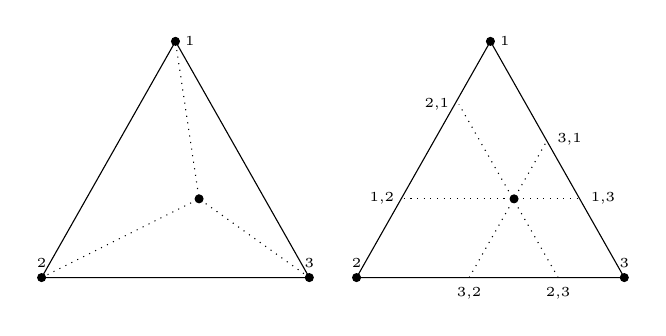
\begin{tikzpicture}
  \draw (0, 0) -- (1.7,3) -- (3.4, 0) -- (0, 0) ;
  \draw[fill] (1.7, 3) circle [radius=0.05] node[anchor=west] {\tiny 1};
  \draw[fill] (0, 0) circle [radius=0.05] node[anchor=south] {\tiny 2};
  \draw[fill] (3.4, 0) circle [radius=0.05] node[anchor=south] {\tiny 3};
  \draw[fill] (2, 1) circle [radius=0.05];
  \draw[dotted] (0,0) -- (2,1) -- (1.7,3);
  \draw[dotted] (3.4, 0) -- (2,1);

  \draw (4, 0) -- (5.7,3) -- (7.4, 0) -- (4, 0) ;
  \draw[fill] (5.7, 3) circle [radius=0.05] node[anchor=west] {\tiny 1};
  \draw[fill] (4, 0) circle [radius=0.05] node[anchor=south] {\tiny 2};
  \draw[fill] (7.4, 0) circle [radius=0.05] node[anchor=south] {\tiny 3};
  \draw[fill] (6, 1) circle [radius=0.05];

  \draw[dotted] (4.6, 1) node[anchor=east] {\tiny 1,2}
  -- (6.85,1) node[anchor=west] {\tiny 1,3};
  \draw[dotted] (5.43, 0) node[anchor=north] {\tiny 3,2}
  -- (6.425, 1.75) node[anchor=west] {\tiny 3,1};
  \draw[dotted] (6.56, 0) node[anchor=north] {\tiny 2,3}
  -- (5.3, 2.2) node[anchor=east] {\tiny 2,1};

\end{tikzpicture}
\caption{Barycentric coordinates. Left: Area opposite of each vertex.
Right: Intersection of lines parallel with triangle edges.}
\label{fig:bary}
\end{figure}
Barycentric coordinates are in fact a special kind of affine coordinates.
Barycentric coordinates are real numbers $\beta_1, \beta_2, \beta_3$ such that
$\sum^3_{i=1} \beta_i = 1$. Given a triangle with vertices $\mathbf v_1,
\mathbf v_2, \mathbf v_3$, the corresponding vertex is given by $\mathbf v =
\sum^3_{i=1} \beta_i \mathbf v_i$. Given $\mathbf v$ and $\mathbf v_i$,
$\beta_i$ can be found by e.g. solving the linear system of
$\beta_1 + \beta_2 + \beta_3 = 1$ and $\mathbf v = \sum^3_{i=1} \beta_i \mathbf
v_i$. $\beta_i$ are all positive on the interior of the triangle. If a point
lies on an edge opposite vertex $i$, then $\beta_i$ is zero.
(If it lies beyond the edge, then $\beta_i < 0$.)

There are two geometric interpretations of barycentric coordinates that will be
useful, as depicted in Figure \ref{fig:bary}. One is that $\beta_i$ is the area
of the smaller triangle opposite $\mathbf v_i$ divided by the area of the large
triangle.
The other is that if a line is placed passing through $\mathbf v$ parallel to
the edge opposite vertex $i$, it will be at $\beta_i$ of the distance between
the edge and its opposite vertex, with $\beta_i = 0$ being on the edge itself.
Let $\mathbf v_{i,j}$ be the point where the line for $i$ meets the line between
vertices $i$ and $j$: then the vertex lies $\frac{\beta_{j}}{1-\beta{i}}$
of the distance from $\mathbf v_{i,j}$ to $\mathbf v_{i,j+1}$. Symbolically,
$\mathbf v_{i,j} = \mathrm{Lerp}(\mathbf v_{j},\mathbf v_i;\beta_{i})$, and
$\mathbf v = \mathrm{Lerp}(\mathrm{Lerp}(\mathbf v_{i-1}, \mathbf v_i;
\beta_{i}), \mathrm{Lerp}(\mathbf v_{i+1}, \mathbf v_i; \beta_{i});
\frac{\beta_{i-1}}{1-\beta_{i}})$ for all $i$.

Generalized barycentric coordinates are defined similarly, but the requirement
that $\sum^3_{i=1} \beta_i = 1$ is dropped. For instance, generalized
barycentric coordinates $\beta'_i$ on the unit sphere replace that requirement
with the condition that $\| \sum^3_{i=1} \beta'_i \mathbf v_i \| = 1$.
$\sum^3_{i=1} \beta'_i$ are $>1$ on the interior of the triangle,
$=1$ on the edges, and $<1$ on the exterior.

\subsection{Dealing with the ellipsoid}
The Earth is reasonably approximated as a sphere, and better approximated as a
slightly flattened oblate ellipsoid. In general this text will only deal with
the spherical approximation, but here we mention two considerations arising
from that approximation.

The vector form described in e.g. \cite{strang12} corresponds to the geodetic latitude.
The mapping between the sphere and the ellipsoid using geodetic latitude is not
area-preserving, conformal, or distance-preserving, although the distortion is
small on the Earth ellipsoid. If applying an area-preserving, conformal, or
distance-preserving map projection, and the required precision is fine enough
that the distortion is a concern, the geodetic latitude can be substituted
with the authalic (equal-area), conformal, or rectifying
(equal-distance along meridians) latitude as described in \cite{snyder87}.
These can be calculated from the geodetic latitude,
and the difference is well-approximated by a Fourier series.

Considering polyhedral maps, in this text we require the edges of the polyhedra
to correspond to geodesics. Geodesics on a sphere are not necessarily geodesics
on an ellipse: as proof, geodesics on an ellipse are not necessarily closed,
while geodesics on a sphere are. (Of course, with the Earth ellipsoid, the
difference between the geodesics is small.) The equator and meridians are
geodesics on both surfaces, so if having exact geodesics is a concern,
place your polyhedron edges along the equator or meridians.

\section{Map projections}

\begin{figure}%[!htbp]
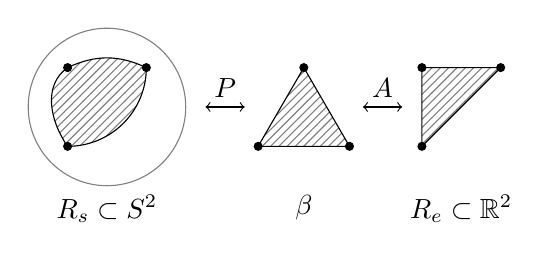
\begin{tikzpicture}
  \draw [gray] (1,1) circle [radius=1];
  \draw[pattern=north east lines, pattern color=gray] (0.5, 0.5) to [out=0, in=-90]
  (1.5, 1.5) to [out=155, in=25]
  (0.5, 1.5) to [out=215, in=125]
  (0.5, 0.5);
  \draw[fill] (0.5,0.5) circle [radius=0.05];
  \draw[fill] (1.5,1.5) circle [radius=0.05];
  \draw[fill] (0.5,1.5) circle [radius=0.05];

  \draw [<->] (2.25,1) -- (2.75,1);
  \draw[pattern=north east lines, pattern color=gray] (2.92, 0.5) -- (4.08, 0.5) -- (3.5, 1.5) -- (2.92, 0.5);
  \draw[fill] (2.92,0.5) circle [radius=0.05];
  \draw[fill] (4.08,0.5) circle [radius=0.05];
  \draw[fill] (3.5,1.5) circle [radius=0.05];

  \draw [<->] (4.25,1) -- (4.75,1);
  \draw[pattern=north east lines, pattern color=gray] (5, 0.5) -- (6, 1.5) -- (5, 1.5) -- (5, 0.5);
  \draw[fill] (5,0.5) circle [radius=0.05];
  \draw[fill] (6,1.5) circle [radius=0.05];
  \draw[fill] (5,1.5) circle [radius=0.05];

\draw (2.5,1) node[anchor=south] {$P$};
\draw (4.5,1) node[anchor=south] {$A$};
\draw (1,0) node[anchor=north] {$R_s \subset S^2$};
\draw (3.5,0) node[anchor=north] {$\mathbf{\beta}$};
\draw (5.5,0) node[anchor=north] {$R_e \subset \mathbb{R}^2$};
\end{tikzpicture}
\caption{Schematic for the application of most projections listed in this text.
$P$ indicates the projection and $A$ is an affine transformation.}
\label{fig:schematic}
\end{figure}

Figure \ref{fig:schematic} illustrates the general form of application of most
projections in this text. (Exceptions are noted in the relevant sections.) The
transformation from barycentric coordinates to the plane, or from $uv$
coordinates to a quadrilateral, takes the same form for each projection, so in
this section we can ignore that part except when there are special
considerations.

The polygon on the sphere $R_s$ and the polygon in the plane $R_e$ can be
basically anything, within the operating parameters of the projection and any
special considerations that may apply. Even with respect to each other, one
can be regular while the other is irregular, if that is desirable. Of course,
this will influence the conformal and length distortion of the projection.

The flip side of this freedom is that given an irregular $R_s$ there is not
necessarily a single recommended way to choose $R_e$. One choice is to choose
$R_e$ such that its edges are proportional in length to those of $R_s$. Another
is to reduce conformal distortion at the vertices. Assuming the maximum angle
distortion $\omega$ is defined at a vertex, $\omega$ is equal to the difference
in the interior angle of that vertex on $R_s$ minus that on $R_e$. Let
$E = \alpha + \beta + \gamma - \pi$ be the spherical excess. To minimize
$\omega$ at each vertex, make the new angles $\alpha' = \alpha - \frac{E}{3}$
and similarly for $\beta'$ and $\gamma'$. This does not define the size of the
triangle, but one can choose $R_e$ to have these angles and the same area of
$R_s$, or that one particular edge has the same length of that in $R_s$, or
another desired quality.

\subsection{Gnomonic}
The gnomonic projection was known to the ancient Greeks, and is the simplest
of the transformations listed here.\cite{snyder87} It has the property that
arcs of great circles are transformed into lines on the plane and vice versa:
that is, geodesics stay geodesics, and (spherical) polygons stay polygons. This
projection is called Method 1 in geodesic dome terminology.\cite{kenner} The
main downside of the gnomonic projection is heavy distortion away from the
center of the projection.

We'll describe this projection in vector form, which is a little unconvential
but will allow us to compare it to other projections later.
Let $\mathbf p$ be a point on a plane given in Hessian normal form by
$\hat{\mathbf n} \cdot \mathbf p = r$. $r$ can be any value except 0.
The gnomonic projection can be described as so:
\begin{equation}
  \widetilde{\mathbf v} = \mathbf p
\end{equation}
\begin{equation}
\mathbf p = \frac{r}
  {\hat{\mathbf n} \cdot \hat{\mathbf v}}\hat{\mathbf v}
\end{equation}
Projection from Euclidean space to the sphere is literally just
normalizing the vector.

For triangles, this projection can be expressed directly in terms
of barycentric coordinates.
\begin{equation}
   \widetilde{\mathbf v} =
   \beta_1 \mathbf v_1 + \beta_2 \mathbf v_2 + \beta_3 \mathbf v_3
\end{equation}
where $\beta_i$ are (planar) barycentric coordinates. If the generalized coordinates are $\beta^\prime_i$, then $\beta^\prime_i = \frac{\beta_1}
{\|\beta_1 \mathbf v_1 + \beta_2 \mathbf v_2 + \beta_3 \mathbf v_3\|}$.

For the inverse, solve this linear system:
\begin{equation}
  \begin{bmatrix}
  \mathbf v_1 & \mathbf v_2 & \mathbf v_3 \end{bmatrix}
   \mathbf{\beta'} = \hat{\mathbf v}
\end{equation}
where $\mathbf{\beta'}$ is a
vector of generalized barycentric coordinates. Then obtain $\mathbf{\beta}$ as
$\mathbf{\beta} = \frac{\mathbf{\beta'}}{\sum{\beta'_i}}$.

\subsection{Conformal triangular}
\begin{figure}%[!htbp]
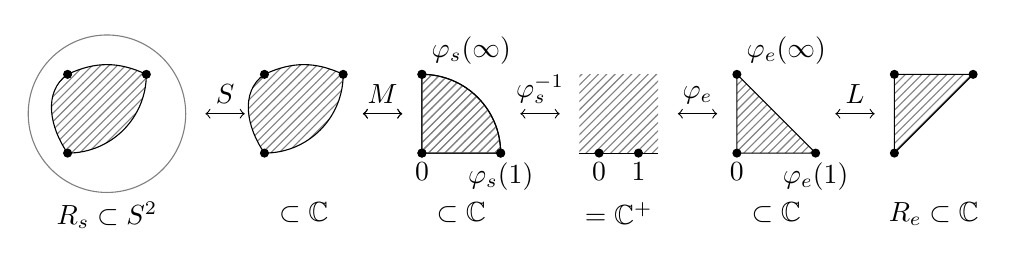
\begin{tikzpicture}
  \draw [gray] (1,1) circle [radius=1];
  \draw[pattern=north east lines, pattern color=gray] (0.5, 0.5)
    to [out=0, in=-90]
  (1.5, 1.5) to [out=155, in=25]
  (0.5, 1.5) to [out=215, in=125]
  (0.5, 0.5);
  \draw[fill] (0.5,0.5) circle [radius=0.05];
  \draw[fill] (1.5,1.5) circle [radius=0.05];
  \draw[fill] (0.5,1.5) circle [radius=0.05];

  \draw [<->] (2.25,1) -- (2.75,1);
  \draw[pattern=north east lines, pattern color=gray] (3, 0.5) to [out=0, in=-90]
  (4, 1.5) to [out=155, in=25]
  (3, 1.5) to [out=215, in=125]
  (3, 0.5);
  \draw[fill] (3,0.5) circle [radius=0.05];
  \draw[fill] (4,1.5) circle [radius=0.05];
  \draw[fill] (3,1.5) circle [radius=0.05];

  \draw [<->] (4.25,1) -- (4.75,1);
  \draw[pattern=north east lines, pattern color=gray] (5, 0.5) --
  (6, 0.5) to [out=90, in=0]
  (5, 1.5) --  (5, 0.5);
  \draw[fill] (5,0.5) circle [radius=0.05];
  \draw[fill] (6,0.5) circle [radius=0.05];
  \draw[fill] (5,1.5) circle [radius=0.05];

  \draw [<->] (4.25,1) -- (4.75,1);
  \draw[pattern=north east lines, pattern color=gray] (5, 0.5) --
  (6, 0.5) to [out=90, in=0]
  (5, 1.5) --  (5, 0.5);
  \draw[fill] (5,0.5) circle [radius=0.05] node[anchor=north] {0};
  \draw[fill] (6,0.5) circle [radius=0.05] node[anchor=north] {$\varphi_s(1)$};
  \draw[fill] (5,1.5) circle [radius=0.05] node[anchor=south west] {$\varphi_s(\infty)$};

  \draw [<->] (6.25,1) -- (6.75,1);
  \fill[pattern=north east lines, pattern color=gray]
    (7,0.5) rectangle (8,1.5);
  \draw (7, 0.5) -- (8, 0.5);
  \draw[fill] (7.25,0.5) circle [radius=0.05] node[anchor=north] {0};
  \draw[fill] (7.75,0.5) circle [radius=0.05] node[anchor=north] {1};

  \draw [<->] (8.25,1) -- (8.75,1);
  \draw[pattern=north east lines, pattern color=gray] (9, 0.5) --
  (10, 0.5) --  (9, 1.5) --  (9, 0.5);
  \draw[fill] (9,0.5) circle [radius=0.05] node[anchor=north] {0};
  \draw[fill] (10,0.5) circle [radius=0.05] node[anchor=north] {$\varphi_e(1)$};
  \draw[fill] (9,1.5) circle [radius=0.05] node[anchor=south west] {$\varphi_e(\infty)$};

  \draw [<->] (10.25,1) -- (10.75,1);
  \draw[pattern=north east lines, pattern color=gray] (11, 0.5) --
  (12, 1.5) --  (11, 1.5) --  (11, 0.5);
  \draw[fill] (11,0.5) circle [radius=0.05];
  \draw[fill] (12,1.5) circle [radius=0.05];
  \draw[fill] (11,1.5) circle [radius=0.05];

\draw (2.5,1) node[anchor=south] {$S$};
\draw (4.5,1) node[anchor=south] {$M$};
\draw (6.5,1) node[anchor=south] {$\varphi^{-1}_s$};
\draw (8.5,1) node[anchor=south] {$\varphi_e$};
\draw (10.5,1) node[anchor=south] {$L$};

\draw (1,0) node[anchor=north] {$R_s \subset S^2$};
\draw (3.5,0) node[anchor=north] {$\subset \mathbb{C}$};
\draw (5.5,0) node[anchor=north] {$\subset \mathbb{C}$};
\draw (7.5,0) node[anchor=north] {$= \mathbb{C}^+$};
\draw (9.5,0) node[anchor=north] {$\subset \mathbb{C}$};
\draw (11.5,0) node[anchor=north] {$R_e \subset \mathbb{C}$};

\end{tikzpicture}
\caption{Schematic of the conformal triangular projection. $S$ is the stereographic
projection, $M$ is a M\"obius transformation, $\varphi$ is the Schwarz triangle
function, $\mathbb{C}^+$ is the complex upper half-plane,
and $L$ is a complex affine transformation.}
\label{fig:conformal}
\end{figure}

Here we take a turn, as this mapping is very different from the others and
uses its own notation. Conformal map projections have deep connections to the
theory of complex functions. Here we introduce a number of functions which
will later be composed together as illustrated in Figure \ref{fig:conformal}.

The stereographic projection $S$ is the conformal map projection between the
Riemann sphere $\mathbb{C} \cup \{\infty\}$ and the sphere $S^2$. Let
$\mathbf{\hat{v}}_0$ designate the center point of the projection, to be
mapped to 0 in the complex plane. Then $\zeta = S\left(\mathbf{\hat{v}}_0;
\mathbf{\hat{v}}\right)$. As the stereographic projection is one of the most
common projections, its formula will not be repeated here: see \cite{snyder87}
if needed. For numerical reasons, the center point should be chosen to avoid
transforming any points within the spherical triangle to the point at infinity
on the Riemann sphere. That can be the centroid of the triangle, or (for
triangles less than a hemisphere) any vertex of the triangle.

A M\"obius transformation is a function of the form
\begin{equation}\begin{split}
  M(z) = \frac{az+b}{cz+d}
\end{split}\end{equation}
where $a, b, c, d$ are complex numbers such that $ad - bc \ne 0$. Note the
similarity between this function and the homographies mentioned earlier: a
M\"obius transformation is in fact a homography of the Riemann sphere,
although on the Riemann sphere that means that circles and lines are mapped to
circles and lines. (Some lines may be mapped to circles, or vice versa.) The inverse of $M(z)$ is $M^{-1}(z) = \frac{dz-b}{-cz+a}$. A M\"obius transformation may be specified by the transformation of three complex numbers $z_1, z_2, z_3$ to $\zeta_1, \zeta_2, \zeta_3$. Assuming all of these values are finite, the M\"obius transformation has coefficients as so:
\begin{equation}a=\det \begin{pmatrix} z_1\zeta_1 & \zeta_1 & 1 \\
    z_2\zeta_2 & \zeta_2 & 1 \\   z_3\zeta_3 & \zeta_3 & 1 \end{pmatrix},\,
  b=\det \begin{pmatrix} z_1\zeta_1 & z_1 & \zeta_1 \\
    z_2\zeta_2 & z_2 & \zeta_2 \\   z_3\zeta_3 & z_3 & \zeta_3 \end{pmatrix},\,
  c=\det \begin{pmatrix} z_1 & \zeta_1 & 1 \\   z_2 & \zeta_2 & 1 \\
    z_3 & \zeta_3 & 1 \end{pmatrix},\,
  d=\det \begin{pmatrix} z_1\zeta_1 & z_1 & 1 \\
    z_2\zeta_2 & z_2 & 1 \\   z_3\zeta_3 & z_3 & 1 \end{pmatrix}
\end{equation}

The Schwarz triangle function conformally transforms the upper
half-plane to a triangle whose edges are circular arcs. It is given by:
\begin{equation}
   \varphi(\alpha,\beta,\gamma; z) = z^{1-c} \frac{_2 F_1(a',b';c';z)}{_2 F_1(a,b;c;z)}
\end{equation}
where $_2 F_1(a,b;c;z)$ is the hypergeometric function and
\begin{equation}\begin{split}
   a & = \frac{1 - \alpha + \beta - \gamma}{2}\\
   b & = \frac{1 - \alpha - \beta - \gamma}{2}\\
   c & = 1 - \alpha\\
   a' &= \frac{1 + \alpha + \beta - \gamma}{2} = 1 + a - c\\
   b' &= \frac{1 + \alpha - \beta - \gamma}{2} = 1 + b - c\\
   c' &= 1 + \alpha
\end{split}\end{equation}
and the angles at each vertex of the triangle are $\pi \alpha, \pi \beta,
\pi \gamma$. (The angles may be dropped if clear in context.)
If $\alpha + \beta + \gamma < 1$, then the triangle is hyperbolic;
if $=1$ it is Euclidean, and if $>1$ it is spherical.\cite{nehari65}
In this text, the hyperbolic case is not relevant.

The Schwarz triangle map maps the boundary of the half-plane
(i.e. $\mathbb{R} \cup \{\infty\}$, the real projective line)
to the boundary of the triangle. The vertices are the points $z=0$, $1$, and
$\infty$ on that line. The map takes $z=0$ to $0$, $z=1$ to $\varphi(1) =
\frac{\Gamma(c-a) \Gamma(c-b) \Gamma(2-c)}{\Gamma(1-a) \Gamma(1-b) \Gamma(c)}$,
and $z=\infty$ to $\varphi(\infty) = \exp\left(i \pi \alpha \right)
\frac{\Gamma(b) \Gamma(c-a) \Gamma(2-c)}{\Gamma(c) \Gamma(b-c+1) \Gamma(1-a)}$
unless $b=0$ (the Euclidean case),
then $\varphi(\infty) = \exp\left(i \pi \alpha \right)
\frac{\Gamma(a) \Gamma(2-c)}{\Gamma(a-c+1)}$

No closed-form inverse $\varphi^{-1}(z)$ exists in general, even in the
Euclidean case when $b=0$ and the denominator of $\varphi(z)$ is 1.
The function has branch cuts on $(-\infty,0]$ and $[1, \infty)$,
and points are transformed to arbitrarily large values,
so care must be taken performing the numerical inversion. A M\"obius
transformation can be used to estimate initial conditions. The unruliness of this numerical inversion makes it difficult to use in real applications

What remains is to combine all these steps into a conformal map projection
between a Euclidean triangle and a spherical triangle. This is also expressed
with $\varphi(z)$.
\begin{equation}\begin{split}\label{eq:conformal}
  \zeta &= L(\varphi\left(\alpha_e,\beta_e,\gamma_e;
    \varphi^{-1}\left(\alpha_s,\beta_s,\gamma_s;
    M(S(\mathbf{\hat{v}}_0;\mathbf{\hat{v}})) \right)\right)\\
  \hat{v} &= S^{-1}\left(\mathbf{\hat{v}}_0;M^{-1}\left(
    \varphi\left(\alpha_s,\beta_s,\gamma_s;
    \varphi\left(\alpha_e,\beta_e,\gamma_e;L^{-1}(\zeta)\right)\right)
  \right)\right)
\end{split}\end{equation}
where $\alpha_s,\beta_s,\gamma_s$ denotes the angles of the spherical triangle
(over $\pi$), and $\alpha_e, \beta_e, \gamma_e$ denotes the angles of the
Euclidean triangle. $M$ is chosen to map
$S(\hat{v}_1)$ to $0$,
$S(\hat{v}_2)$ to $\varphi\left(\alpha_s,\beta_s,\gamma_s;1\right)$, and
$S(\hat{v}_3)$ to $\varphi\left(\alpha_s,\beta_s,\gamma_s;\infty\right)$.
$L$ is a conformal affine transformation, chosen to map
$0$ to $\zeta_1$,
$\varphi\left(\alpha_e,\beta_e,\gamma_e;1\right)$ to $\zeta_2$, and
$\varphi\left(\alpha_e,\beta_e,\gamma_e;\infty\right)$ to $\zeta_3$.
(Only two of these correspondences are needed to determine $L$.)
In complex terms, $L(z)=az + b$, where a and b are complex constants.

The values on the boundary of the triangle depend on the shape of the entire
triangle. These values are only guaranteed to be equal on the edge between two
triangles if those triangles are reflections of each other across that edge.
That is, those triangles are part of a tiling of the sphere with Schwarz
triangles.%TODO go to the actual source and clarify this

Deriving a general conformal map projection for quadrilaterals and higher
polygons is difficult. While there is only one solution for triangles, for
quadrilaterals there is a one-parameter family of solutions, a two-parameter
for pentagons, and so forth.\cite{nehari57} %TODO cite the right section
Furthermore, except for a few specific cases, the general solution is not a
named function: notable exceptions are the elliptic integral and Jacobi
elliptic functions, which appear in the functions between the square and the
hemisphere.\cite{fong16}
One possible way to handle higher polygons is to divide them into triangles,
but a) if new vertices are introduced, those vertices are singular points,
and b) those triangles must be Schwarz triangles as mentioned above.

\subsection{Snyder equal-area}
The Snyder equal-area projection can be applied to any regular polygon. The
equations in \cite{snyder92} are lengthy, and don't seem to simplify much when
expressed in terms of vectors. The special cases of the hemisphere and the cube
face do have nice simple forms, however.\cite{lambers}\cite{patt} Snyder's
equations won't be repeated here.

The Snyder projection starts by subdividing a regular polygonal face into
isosceles triangles, where two vertices of the new triangles are vertices of
the original polygon, and the third is the center of the polygon. Because of
this interruption, the projection is not differentiable on the lines from the
center to the original vertices. This projection can be applied to faces larger
than a hemisphere, as long as each subdivision triangle is smaller than a
hemisphere.

The Snyder projection does not require the faces of a polyhedron to be the
same, but does require (to maintain the equal-area property between
subdivsions) that the faces be subdividable into identical triangles. In
general, the Snyder equal-area projection cannot be adapted to irregular
polygons while maintaining the equal-area property and not introducing extra
lines of interruption. However, if a polyhedra is made up of identical
isosceles triangles, and those triangles meet at appropriate edges, the map can
be applied directly to those faces without subdivision. (Isosceles triangles of
different dimensions may be allowed if one is willing to abandon either the
equal-area property holding between different faces or the polygons on the
plane fitting together into a net.) An example of an irregular polyhedra that
can be used in this way is an $n$-bipyramid, formed by gluing two $n$-sided
pyramids together at the $n$-gonal base. (This is effectively the same as
applying the subdivision method to a $n$-dihedron.) Other polyhedra would
include the (regular) icosahedron and octahedron and the tetragonal disphenoid
(a stretched form of a tetrahedron with isosceles faces, of which the regular
tetrahedron is a subtype).

\subsection{Spherical areal}
This projection is an analogy with the relationship of barycentric coordinates
to area. Treat $\beta_i$ as the proportion of spherical area in the triangle
that is opposite the vertex $\hat{\mathbf v}_i$. Let $\Omega$ be the spherical
area (solid angle) of the spherical triangle and $\Omega_i = \beta_i\Omega$ be
the area of the smaller triangle opposite vertex $\hat{\mathbf v}_i$.
This area can be found in terms of vectors using this formula:\cite{oosterom}\cite{eriksson}
\begin{equation}
\tan(\Omega/2) = \frac{|\mathbf{\hat{v}_1} \cdot
       \mathbf{\hat{v}}_2 \times \mathbf{\hat{v}}_3|}
       {1+\mathbf{\hat{v}}_1\cdot \mathbf{\hat{v}}_2+\mathbf{\hat{v}}_2
       \cdot \mathbf{\hat{v}}_3+\mathbf{\hat{v}}_3\cdot \mathbf{\hat{v}}_1}
\end{equation}

The formula to find $\hat{\mathbf v}$ given $\beta_i$ more complicated,
although it's also derived from the formula for spherical area.

%https://math.stackexchange.com/questions/1151428/point-within-a-spherical-triangle-given-areas/3189416#3189416

\begin{equation}
\label{eq:sphareal}
  \begin{split}
  \mathbf G & \hat{\mathbf v} = \mathbf h \\
   \mathbf G & = \begin{bmatrix}
   \mathbf g_1 & \mathbf g_2 & \mathbf g_3 \end{bmatrix} \\
   \mathbf h & = \begin{bmatrix} h_1  & h_2 & h_3  \end{bmatrix}^T \\
   \mathbf g_{i} & = \left(1+\cos \Omega_{i}\right) \mathbf v_{i-1} \times
   \mathbf v_{i+1} - \sin\Omega_{i}\left(\mathbf v_{i-1} +
   \mathbf v_{i+1}\right)\\
   h_i &= \sin\Omega_i\left(1+\mathbf v_{i-1}\cdot\mathbf v_{i+1}\right)
\end{split}\end{equation}
The subscripts loop around: 0 should be interpreted as 3, and 4 should be
interpreted as 1. To clarify, $\mathbf G$ is the 3x3 matrix where the $i$th
column is $\mathbf g_i$, and $\mathbf h$ is the column vector where the
$i$th element is $h_i$. The vector $\hat{\mathbf v}$
can be solved for using standard matrix methods.

OR:
\begin{equation}\begin{split}
\tau   &= \tan\left(\frac{\Omega}{2}\right) \\
\tau_i &= \tan\left(\frac{\Omega_i}{2}\right) \\
t_i &= \frac{\tau_i}{\tau} \\
a_i &= \mathbf v_{i-1} \cdot \mathbf v_{i+1} \\
b_i &= \frac{a_{i-1} + a_{i+1}}{1 + a_i} \\
c_i &= \frac{t_i}{(1+b_i) + (1-b_i) t_i} \\
f_i &= \frac{c_i}{1 - c_1 - c_2 - c_3} \\
\mathbf v &= \sum f_i \mathbf v_i = \frac{\sum c_i \mathbf v_i }{ 1 - \sum c_i }
\end{split}\end{equation}

\subsection{Fuller}
this entire section needs to be reworked\cite{crider08}
\begin{figure}%[!htbp]
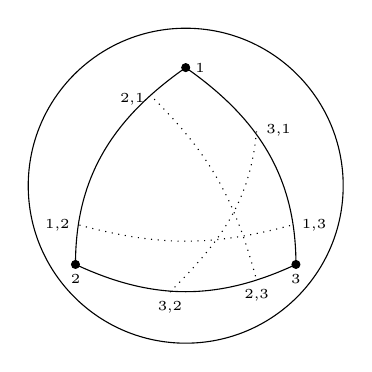
\begin{tikzpicture}
  \draw (2,2) circle [radius=2];

  \draw (0.6, 1) to [out=-25, in=205]
  (3.4, 1) to [out=90, in=-35]
  (2, 3.5) to [out=215, in=90]
  (0.6, 1);
  \draw[fill] (2, 3.5) circle [radius=0.05] node[anchor=west] {\tiny 1};
  \draw[fill] (0.6, 1) circle [radius=0.05] node[anchor=north] {\tiny 2};
  \draw[fill] (3.4, 1) circle [radius=0.05] node[anchor=north] {\tiny 3};
  \draw[dotted] (0.65, 1.5)  node[anchor=east] {\tiny 1,2}
  to [out=-15, in=195] (3.35, 1.5) node[anchor=west] {\tiny 1,3};

  \draw[dotted] (1.8, 0.65) node[anchor=north] {\tiny 3,2}
  to [out=45, in=265] (2.9, 2.7) node[anchor=west] {\tiny 3,1};
  \draw[dotted] (1.6, 3.1) node[anchor=east] {\tiny 2,1}
  to [out=-45, in=105] (2.9, 0.8) node[anchor=north] {\tiny 2,3};
\end{tikzpicture}
\caption{Intersection of great circle arcs inside a spherical triangle,
and the small spherical triangle formed by the arcs. Exaggerated so that the
small triangle is visible; not to scale.}
\label{fig:intlines}
\end{figure}
note similiarities between chamberlin and fuller, as per \cite{gray94}

This is Method 2 in geodesic dome terminology. Recall in our earlier discussion
of barycentric coordinates that on a plane triangle, we can draw a line
corresponding to each $\beta_i$, and those three lines meet at a point. On the
sphere, if we make the same construction, the lines do not meet at a point
(except on the edges), but instead intersect to form a small spherical
triangle. Take a point within that triangle as $\mathbf v$.
Typically the centroid is used, as it's easy to calculate,
although we'll discuss another variation.

In analytic terms, use Slerp to determine the points on each triangle edge.
Take the cross product of the opposing pairs of points to determine the normal
to the intersecting plane corresponding to each line. Take the cross product of
each pair of normals to find a vector proportional to the point of
intersection. (As the cross product is antisymmetric, be careful about order
here.) Then normalize each vector and take their centroid.

In terms of equations, Method 2 or the Great Circle Intersection
method on a triangle is:
\begin{equation}\begin{split}%??? does this reduce to slerp on the edges?
\widetilde{\mathbf v} & = \sum^3_{i=1} \frac{\mathbf h_i \times \mathbf h_{i+1}}
{\|\mathbf h_i \times \mathbf h_{i+1}\|} \\
\mathbf h_i & =
\mathrm{Slerp}(\mathbf v_{i-1}, \mathbf v_i; \beta_{i})
\times
\mathrm{Slerp}(\mathbf v_{i+1}, \mathbf v_i; \beta_{i})
\end{split}\end{equation}

No explicit inverse, unlike \cite{gray95}\cite{crider08}

The above equation can be tweaked slightly by removing the step of normalizing
the vectors at the points of intersection. This still produces a point within
the triangle. This formula is a little more computationally efficient and
easier to treat algebraically. Where $\mathbf h_i$ is as before:
\begin{equation}\label{eq:gct}%??? does this reduce to slerp on the edges?
\widetilde{\mathbf v} = \sum^3_{i=1} \mathbf h_i \times \mathbf h_{i+1} \\
\end{equation}

This method can be extended to the Quadrilateral. Use Slerp to find points on
opposing sides of the quadrilateral, use the cross product to find their
normal, and then use the cross product to find the point of intersection. Since
we draw two intersecting lines, there is only one point of intersection within
the quadrilateral. The formula is:
\begin{equation}\label{eq:gcq}%??? does this reduce to slerp on the edges?
\widetilde{\mathbf v} =
(\mathrm{Slerp}(\mathbf v_1, \mathbf v_2; \frac{u+1}{2})
\times
\mathrm{Slerp}(\mathbf v_4, \mathbf v_3; \frac{u+1}{2}))
\times
(\mathrm{Slerp}(\mathbf v_1, \mathbf v_4; \frac{v+1}{2})
\times
\mathrm{Slerp}(\mathbf v_2, \mathbf v_3; \frac{v+1}{2}))
\end{equation}

This is similar to the Great Circle method, except instead of using the great
circles to calculate the intersections of the lines, we use another spherical
linear interpolation to get a point near the intersection. We effectively use
the Lerp formulas from the section on coordinates, substituting Slerp for Lerp.
Unlike Lerp, Slerp does not commute, so we take the different permutations of
the arguments and combine the different points that result.

Triangular:
\begin{equation}\label{eq:fullert}
\widetilde{\mathbf v} = \sum^3_{i=3} \mathrm{Slerp}(
\mathrm{Slerp}(\mathbf v_{i-1}, \mathbf v_i; \beta_{i}),
\mathrm{Slerp}(\mathbf v_{i+1}, \mathbf v_i; \beta_{i});
\frac{\beta_{i-1}}{1-\beta{i}})
\end{equation}
Quadrilateral:%??? not symmetric?
\begin{equation}\label{eq:fullerq}
  \begin{split}
\widetilde{\mathbf v} =& \mathrm{Slerp}(
\mathrm{Slerp}(\mathbf v_1, \mathbf v_2; \frac{u+1}{2}),
\mathrm{Slerp}(\mathbf v_4, \mathbf v_3; \frac{u+1}{2}); \frac{v+1}{2})\\
&+ \mathrm{Slerp}(
\mathrm{Slerp}(\mathbf v_1, \mathbf v_4; \frac{v+1}{2}),
\mathrm{Slerp}(\mathbf v_2, \mathbf v_3; \frac{v+1}{2}); \frac{u+1}{2})
\end{split}
\end{equation}

(or is this forward fuller and the other one's reverse fuller?)

Solve for each $\beta'_i$:
\begin{equation}
\begin{vmatrix} \mathbf v &
\mathrm{Slerp}(\mathbf v_{i-1}, \mathbf v_i; \beta'_i) &
\mathrm{Slerp}(\mathbf v_{i+1}, \mathbf v_i; \beta'_i) \end{vmatrix} = 0
\end{equation}
$\beta_i$ does not have a closed-form solution on general triangles,
but each $\beta_i$ can be optimized separately,
so the optimization process is not too unwieldy.

In general, $\sum \beta'_i \ne 1$ for the $\beta'_i$ resulting from this
process. Let $\beta_i = \frac{\beta'_i }{\sum \beta_i}$.

\subsection{Naive Slerp}
The Naive Slerp method is derived by a naive analogy with spherical linear
interpolation (Slerp) extended to barycentric or $uv$ coordinates, thus the
name.
\subsubsection{Triangles}
\begin{equation}\label{eq:nst}
   \widetilde{\mathbf v} = \sum_{i=1}^3\frac{\sin(w\beta_i)}{\sin(w)}  \mathbf v_i
\end{equation}
Here, $w$ is a function of $\beta_i$. Let $w_i$ be the spherical length of the edge opposite vertex $i$. Then,
\begin{equation}
  w = \frac{\beta_0 \beta_1 w_2 + \beta_1 \beta_2 w_0 + \beta_2 \beta_0 w_1}
      {\beta_0 \beta_1 + \beta_1 \beta_2 + \beta_2 \beta_0}.
\end{equation}
This function satisfies the requirement that $w = w_i$ on the edge opposite
vertex $i$, and elsewhere on the triangle smoothly parameterizes between the
values. $w$ is not defined at the vertices, and does not have a limit there
unless the two edges that meet at that vertex have the same length. However,
any positive value for $w$ can be used there without changing the result.
If all the edges are equal length,
$w$ can be replaced with that constant edge length.

\subsubsection{Projection of $\widetilde{\mathbf v}$}
The naive slerp methods produces unit vectors along the edges. Because the
projected edges already lie on the sphere, we have freedom in how to adjust
$\widetilde{\mathbf v}$ to lie on the sphere. The easiest is just to centrally
project the vertices, that is, to normalize $\widetilde{\mathbf v}$ like we
have been. Another option is to perform a parallel projection along the
face normal, as defined earlier. We need the parallel distance $p$ from the
vertex to the sphere surface in the direction of the face normal
$\hat{\mathbf n}$, such that $\hat{\mathbf v} =
\widetilde{\mathbf v} + p\hat{\mathbf n}$. $p$ is given by:
\begin{equation}
   p = -\widetilde{\mathbf v} \cdot \hat{\mathbf n} +
   \sqrt{1+\widetilde{\mathbf v} \cdot \hat{\mathbf n}-\widetilde{\mathbf v} \cdot \widetilde{\mathbf v}}
\end{equation}
$p$ can also be approximated as $\widetilde{p} = 1 - \|\widetilde{\mathbf v}\|
\leq p$, which takes fewer operations and doesn't require
calculation of the face normal. Technically, you can project in almost any
direction, not just that of the face normal, but most other choices don't
produce a symmetric result.

Really, the projection can be performed from any point in space. Central
projection uses rays from a point at the center of the sphere, and parallel can
be thought of as using rays from a point at infinity. Instead of specifying the
point, we define a linear combination of the two projections:
\begin{equation}
  \hat{\mathbf v} = \frac{\widetilde{\mathbf v} + kp\mathbf c}{\|\dots\|}
\end{equation}
When $k=0$, that's the central projection: when $k=1$, it's the parallel
projection. $p$ may be replaced by $\widetilde{p}$. If our goal is to optimize
a measurement of the map projection, like conformal or area distortion, we
can do a 1-variable optimization on $k$.

\subsection{Linear combination}

Let $f_i (\mathbf v)$ be a sequence of map projections from a spherical
polygon $R_s$
to a spherical polygon $R_e$.
Let $\mathbf v_i$ be the
vertices of the spherical polygon. Furthermore, require that $f_i(\mathbf v_j)$
takes the same value for all $i$ and $j$: the projections all maintain the same
orientation of polygon. Then, let $w_i$ be a sequence of weights, possibly
negative, such that $\sum w_i = 1$. It can be easily demonstrated that
$g(\mathbf v) = \sum w_i f_i(\mathbf v)$ is also a map projection from $R_s$ to
$R_e$. (This holds whether we think of $R_e$ in terms of barycentric coordinates
or a planar Euclidean polygon.)

If any individual $f_i(\mathbf v)$ is non-differentiable or has a singularity
at any point or points, $g(\mathbf v)$ will generally be non-differentiable or
have a singularity in the same place.

Unfortunately, $g(\mathbf v)$ may not have a closed-form inverse, even if all
of the contributing $f_i(\mathbf v)$ do.

\section{Analysis}
\subsection{From the sphere to the plane}

\subsection{From the plane to the sphere}

\section{Conclusion}

\bibliographystyle{plain}
\bibliography{references}

\end{document}
